\chapter{Introdução}
\label{chap:Introdução}

Uma tendência que tem ganhado força na área de redes de sensores sem fio é o uso de nós sensores heterogêneos. Este nós podem ser utilizados como ferramentas para se cumprir os requisitos de sofisticadas aplicações emergentes, tais como sistemas de monitoramento \cite{Freitas20092}.

Uma maneira simples de se monitorar áreas de interesse é espalhar sensores por toda sua extensão. Contudo, um dos maiores desafios no desenvolvimento de tais aplicações em redes de sensores encontra-se em como prover coordenação entre os nós envolvidos, atentendendo assim, às necessidades dos usuários \cite{Mhatre2005}.

Este trabalho apresenta uma investigação de estratégias para coordenar um conjunto de nós sensores terrestres estáticos (posicionados no solo) e de \uavs (\emph{Unmanned Aerial Vehicles} - UAV) que carregam uma variedade de sensores. Esta coordenação tem como objetivo prover monitoramento e detecção eficientes de intrusos em uma determinada área de interesse. Preocupações como economia de energia, latência e largura de banda são exploradas para que se alcance um monitoramento eficiente considerando-se as limitações e desafios de uma rede de sensores sem fio.

Dentre as estratégias utilizadas, destacam-se as técnicas de Auto-Organização Emergente, que se apresentam como técnicas que não utilizam controles externos ou centrais. Em sistemas auto-organizados, as entidades individuais interagem entre si localmente. Porém, pelas interações locais, promovem um comportamento global emergente.

Diversos nós sensores são distribuídos em uma área de interesse, bem como são distribuídos estrategicamente \vants sobrevoando a área de interesse. Os nós sensores terrestres são configurados para acionar alarmes na ocorrência de um dado evento de interesse, isto é, entrada de um intruso na área, enquanto os \vants recebem os alarmes e têm que decidir qual \vant é o mais hábil a tratar o alarme acionado.

O sistema proposto por este trabalho é projetado para que os nó sensores e \vants se comuniquem e tomem decisões autonomamente, isto é, sem nenhum controle externo ou centralizado. Ao fim, é gerado um comportamento global emergente a partir das pequenas interações entre os indvíduos do sistema (nós sensores e UAVs).


%%%%%%%%%%%%%%%%%%%%%%%%%%%%%%%%%%%%%%%%%%%%%%%%%%%%%%%%%%%%%%%%%%%%%%%%%%%%%%%%%%

\section{Motivação}
\wsn (RSSFs) são utilizadas para se aumentar a eficiência de uma gama de aplicações, tais como detecção de alvos, monitoramento, vigilância ou gerenciamento de desastres. \rssfs utilizando nós sensores estáticos têm sido desesnvolvidas, testadas e utilizadas em diversas aplicações de monitoramento \cite{Mainwaring2002}.

Contudo, nós sensores terrestres apresentam algumas limitações, especificamente, neste caso, em relação ao raio de comunicação de cada nó. O uso de nós sensores móveis em tais situações pode prover melhorias significativas. Nós sensores móveis podem prover habilidades para que a rede possa se adaptar dinamicamente aos eventos ocorridos no ambiente, bem como colaboram para se aumentar a conectividade dentre da rede  \cite{Aware}.

Um nó concentrador estático é geralmente localizado nas extremidades de uma RSSF, todavia, isto geralmente requer uma longa cadeia de troca de mensagens (\emph{multi hop}) para que um nó sensor consiga transmitir uma mensagem para o nó concentrador. Isto resulta em baixo desempenho do sistema, uso ineficiente da energia e desperdício de largura de banda \cite{Chang2007}.

Neste contexto, tem-se a possibilidade de utilização de UAVs como nós sensores móveis em uma RSSF. Autores como \cite{Lucchi2007} têm considerado o uso de nós sensores terrestres espalhados por uma área de interesse. Estes nós podem coletar diversos tipos de informação do ambiente, tais como temperatura, pressão, umidade, etc, e possuem a capacidade de se comunicar com o \vant no momento em que a aeronave sobrevoa as áreas onde os nós se encontram posicionados.

O uso de \vants como sensores móveis da rede pode prover a habilidade de se monitorar os eventos ocorridos em uma maior granularidade. Os nós sensores podem detectar a ocorrência de um evento, porém podem não conter recursos suficientes para análises mais detalhadas, passando assim a ocorrência a um \vant com habilidades específicas para tratar o problema.

Neste contexto é que o presente trabalho propõe técnicas para a coordenação de uma \rssf heterogênea. O cenário principal é a distribuição de milhares de sensores terrestres simples e de pouca capacidade computacional, utilizados somente para a detecção de eventos de interesse e algumas poucas aeronaves não tripuladas especializadas no tratamento de diferentes eventos. Detectados os eventos, os nós sensores devem se coordenar e garantir que a mensagem seja entregue ao \vant mais hábil para tratar o alarme de ocorrência destes eventos.


\section{Objetivos}

Este trabalho tem por objetivo global desenvolver e aplicar técnicas de coordenação entre nós sensores sem fio e \uavs em uma aplicação de monitoramento e vigilância. Para o alcance deste objetivo serão utilizadas técnicas Auto-Organizáveis para a coordenação e controle da \rssf.

\subsection{Objetivos Específicos}

Este trabalho tem como objetivos específicos:

\begin{description}

	\item [Pesquisa e elaboração de algoritmos de coordenação de nós sensores e \vants:] desenvolvimento de algoritmos para detecção e entrega de alarmes a partir dos nós sensores, desenvolvimento de uma heurística bio-inspirada para localização eficiente do \uav mais próximo e algoritmos para \emph{tracking} e perseguição de intrusos na área.

	\item [Implementação dos algoritmos e técnicas no ambiente de simulação GRUBiX:] implementação de cada um dos algoritmos no ambiente de simulação \emph{open source} GRUBiX, desenvolvidos pelo Grupo de Redes Ubíquas do Departamento de Ciência da Computação da Universidade Federal de Lavras. Adicionalmente, acrescentar melhorias e funcionalidades à atual versão do simulador.

	\item [Comparação entre algoritmos convencionais e os desenvolvidos no trabalho:] comparações quantitativas dos resultados a partir de experimentos computacionais considerando-se cada uma das técnicas em diferentes cenários e configurações.

\end{description}

%%%%%%%%%%%%%%%%%%%%%%%%%%%%%%%%%%%%%%%%%%%%%%%%%%%%%%%%%%%%%%%%%%%%%%%%%%%%%%%%

\section{Descrição do Problema}

Este trabalho preocupa-se em pesquisar e desenvolver estratégias para a coordenação de uma rede de sensores heterogênea. A rede em questão deve ser utilizada para prover tarefas de monitoramento e vigilância de um ambiente de interesse. Como ferramentas para se realizar estas tarefas de monitoramento são utilizados nós sensores terrestres equipados com diversas interfaces de sensoriamento e \vants também equipados com interfaces de sensoriamento e enlaces de comunicação sem fio.

A justificativa e motivação para a utilização destes diferentes tipos de nós sensores encontra-se no fato de que um nó sensor terrestre usual apresenta capacidade computacional reduzida. Portanto, estes tipos de nós são incapazes de cumprir todas as tarefas da rede individualmente. Em contrapartida, estes nós sensores convencionais geralmente possuem custos reduzidos, o que propicia o uso de vários sensores para a realização de missões. 

\uavs podem variar em tamanhos, formas, configurações e propósitos, adequando-se a diversos cenários de aplicação. Neste trabalho, justifica-se o uso de \emph{Mini-UAVs} (UAVs Multi-Missão), que são aeronaves de custo não tão elevado quando comparados aos custos de aeronaves de grande porte. Portanto, uma alternativa interessante é a utilização de \emph{Mini-UAVs} carregando uma variedade de sensores específicos (sensores como câmeras de alta resolução, infra-vermelho, GPS, etc) e que possuam poder computacional superior aos nós sensores terrestres, permitindo assim que os \vants possam realizar missões e medidas mais sensíveis e específicas.

Esta relação entre sensores terrestres simples e de baixo custo e \vants relativamente mais caros justifica o uso de vários sensores simples espalhados pela área de interesse em conjunto com alguns poucos, ou apenas um, \vant para realizar as tarefas mais específicas. Por fim, o problema tratado é o desenvolvimento de estratégias eficientes para detecção de um evento através dos nós sensores mais simples e garantir que as mensagens sejam entregues aos \vants mais hábeis a tratar o evento de forma específica. Adicionalmente, o \vant selecionado deve retornar ao ponto onde o evento foi detectado, ou seguir um rastro, caso o evento ocorrido possua mobilidade.

A próxima subseção demonstra o funcionamento básico do problema.

\subsection{Demonstração do Problema}

Resumidamente, a demonstração do problema pode ser dividida em quatro partes principais:

\begin{description}

	\item[ (a) Distribuição de Ferormônio: ] o \vant sobrevoa continuamente a área de interesse da aplicação. Enquanto sobrevoa esta área, o \vant deve se comunicar com os nós sensores que se encontram abaixo do mesmo, estes nós armazenam um valor com a intensidade do sinal com que a mensagem foi recebida. Neste momento é formado um rastro da aeronave.
	
	\item[ (b) Detecção e Propagação do Evento:] quando um evento é detectado, os nós sensores terrestres devem realizar uma negociação a fim de enviar uma mensagem de alarme para os \vants presentes na área. Esta mensagem deve encontrar o rastro de ferormônio formado em (a) e prosseguir até o \vant mais hábil para tratar o evento ocorrido.

	\item[ (c) \emph{Tracking} e Perseguição do Intruso: ] no momento em que os nós sensores detectam a presença de um dado evento, como exemplo o caso de um intruso, providências devem ser tomadas para que o mesmo alarme de evento não seja repetido. Por exemplo, o nó sensor X percebe a presença de um intruso na área, poucos segundos depois o nó Y também percebe o mesmo intruso, se ambos os nós enviarem um alarme aos \vants pode ocorrer carga excessiva na rede, bem como gerar confusão entre os \vants, pois os mesmos são interrompidos e reprogramados a cada alarme recebido. Portanto, na ocorrência de um evento, os nós da micro região onde onde houve a detecção devem alterar seu modo de trabalho, realizando assim uma perseguição e rastreamento, marcando uma trilha de mobilidade do evento, ao invés de soar os alarmes novamente.

	\item[ (d) Deslocamento do \vant: ] com a percepção de um alarme, o \vant mais hábil deve prosseguir do local onde se encontra para o local de ocorrência do evento, para então tratar ou seguir a trilha do mesmo. Um fato interessante é que a localização dos nós não é absoluta, portanto, um \vant não sabe a localização exata de ocorrência do evento. Como consequência deste fato, o \vant deverá seguir a trilha inversa por onde recebeu a mensagem.

\end{description}

A figura \ref{fig:app} demonstra o funcionamento básico do sistema de monitoramento.

\begin{figure}[h!]
\centering
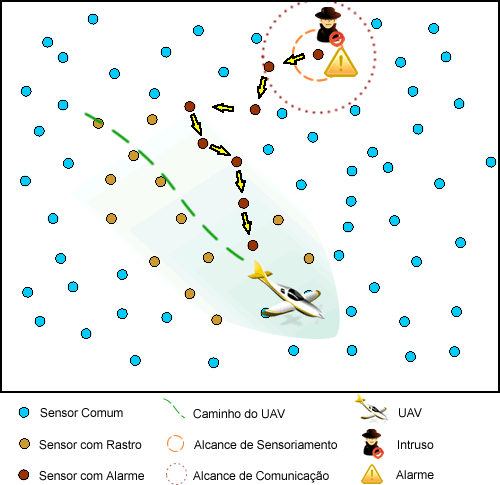
\includegraphics[width=12cm]{pictures/application.png}
\caption{Funcionamento Básico da Aplicação}
 \label{fig:app}
\end{figure}




%%%%%%%%%%%%%%%%%%%%%%%%%%%%%%%%%%%%%%%%%%%%%%%%%%%%%%%%%%%%%%%%%%%%%%%%%%%%%%%%%
\section{Organização do Trabalho}

Este trabalho encontra-se organizado em cinco capítulos. O capítulo \ref{chap:Introdução} apresenta uma introdução, a motivação, os objetivos e definição do problema estudado. No capítulo \ref{chap:Referencial Teórico} podem ser encontradas as definições e bases teóricas para o entendimento do problema. A metodologia para realização do trabalho encontra-se no capítulo \ref{chap:Metodologia}. Os capítulos \ref{chap:Resultados Esperados} e \ref{chap:Cronograma}, respectivamente, são compostos pelos resultados esperados e o cronograma de estudo a ser realizado.


